\section{Aufgabe 2} \label{ex2}
In der Aufgabe 2 wurde eine Fibonacci-Algorithm in c mitgebracht. Der Code wurde mit HLS synthetisiert und sowohl den Ressourcenverbrauch als auch das Timing unseres Codes analysiert.

\subsection{C-Code}
C-Code zur Berechnung des n-ten Wertes F(n) der  Fibonacci-Folge aus den Startwerten F0 = 0 und F1 = 1\\

Fibonacci für Hardware Implementation
\begin{verbatim}
#include "fir.h"

void fir (
  data_t result[20],
  data_t n
  ) {

  int i;
  *result = 0;
  *(result+1) = 1;
  Shift_Accum_Loop: for (i=2;i<20;i++) {
	  *(result+i) =  *(result+i-1) +  *(result+i-2);
  }
}
\end{verbatim}

Testbench
\begin{verbatim}
#include <stdio.h>
#include <math.h>
#include "fir.h"

int main () {
   FILE         *fp;

  data_t signal, output[N];
  //coef_t taps[N] = {2,100,9};

  int i;
  
  fp=fopen("out.dat","w");
  fir(output,N);

  for (i=0;i<N;i++) {
	// Execute the function with latest input
	// Save the results.
    fprintf(fp," the %d-Fibonatchi is =  %d\n",i+1,output[i]);
  }
  fclose(fp);

  printf ("Comparing against output data \n");
  if (system("diff -w out.dat out.gold.dat")) {

	fprintf(stdout, "*******************************************\n");
	fprintf(stdout, "FAIL: The result is not correct\n");
	fprintf(stdout, "*******************************************\n");
     return 1;
  } else {
	fprintf(stdout, "*******************************************\n");
	fprintf(stdout, "PASS: The result is correct!\n");
	fprintf(stdout, "*******************************************\n");
     return 0;
  }
}
\end{verbatim}

\subsection{C-Code Analyse}
Das Bild zeigt den Ressourcenverbrauch und das Timing\\

\begin{minipage}{\textwidth}
    \begin{center}        
        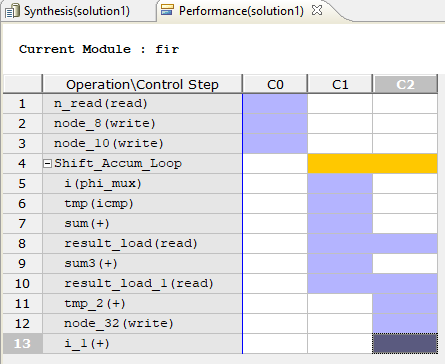
\includegraphics[scale=0.75]{img/Fibo.png} 
    \end{center}
\end{minipage}
\begin{center}
Perfomance in Zyklen
\end{center}

\begin{minipage}{\textwidth}
    \begin{center}        
        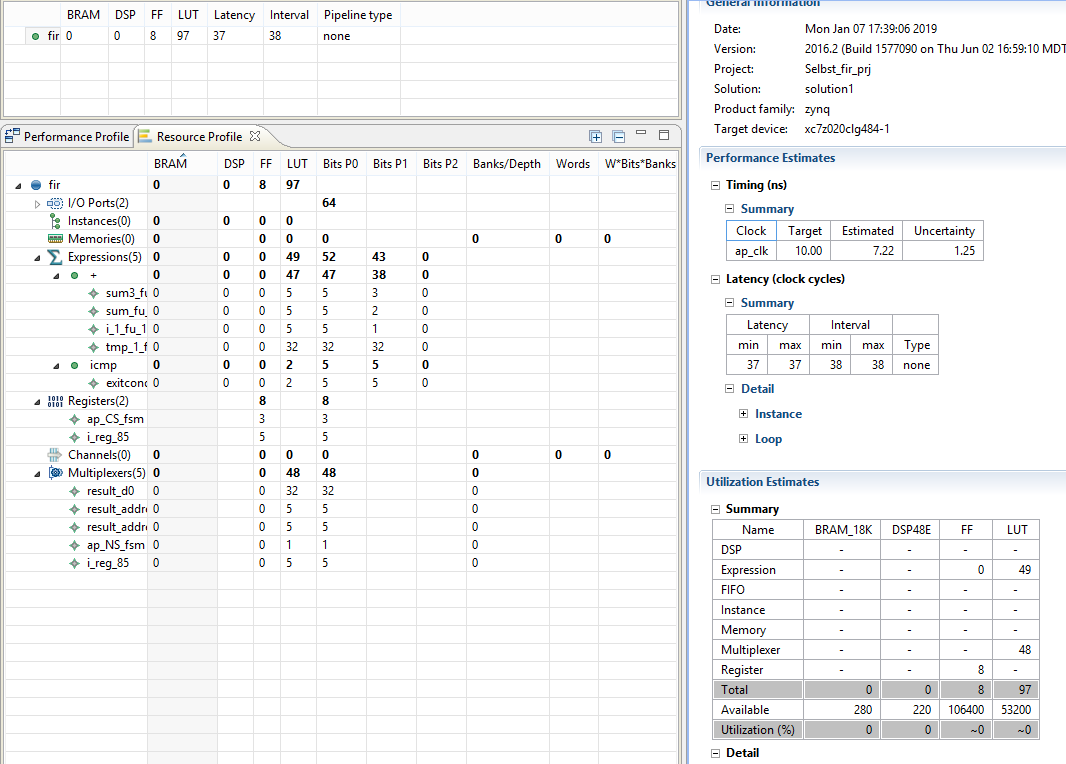
\includegraphics[scale=0.6]{img/fibo1.png} 
    \end{center}
\end{minipage}
\begin{center}
Ressourcenverbrauch 1
\end{center}

\begin{minipage}{\textwidth}
    \begin{center}        
        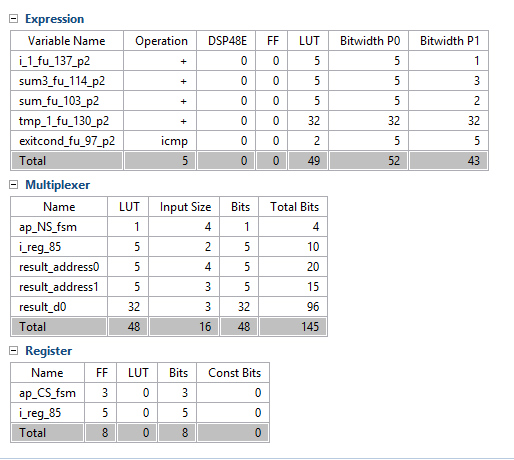
\includegraphics[scale=1.0]{img/fibo2.png} 
    \end{center}
\end{minipage}
\begin{center}
Ressourcenverbrauch 2
\end{center}



